\section{Methodology}

\subsection{Dependant Variables}\label{sec:dependent_variables}


The values for which various sets of HOG parameters will be tested in this investigation are listed in table \ref{table:dependent_variables}. Table \ref{table:dependent_variables} also includes the use of a "holistic" derivative mask, as introduced in section \ref{sec:deriv_mask}, which, while not a component of dimensionality, does change the shape of the feature vector $\vec{L}$.

\begin{table}
\renewcommand{\arraystretch}{1.0}
\begin{tabular}{@{} l @{\hspace{1cm}} l @{}}    
    \toprule
    \emph{Parameter} & \emph{Values}  \\\midrule
    Window Dimension Pairs ($W_h$,$W_w$)             & (100, 50), (128, 96), (128, 64), (112, 48)  \\ 
    Cell Histogram Bin Counts ($\omega$)              & 9, 13, 18  \\ 
    Cell Dimension Pairs ($c_w$,$c_h$)           & (4,4), (6,6), (8,8), (10,10)  \\ 
    Block Dimension Pairs ($b_w$,$b_h$)           & (1,1), (2,2), (3,3), (4,4)  \\ 
    Block Stride Dimension Pairs ($s_w$,$s_h$)              & (1,1), (2,2), (3,3)  \\ 
    Holistic Derivative Mask (appendix \ref{appendix:holistic_der_mask}) & True, False  \\\bottomrule
\end{tabular}
\caption{Dependent variables for the experiment}
\label{table:dependent_variables}
\end{table}

With the only restriction on the dependent variables being $b_w\ge s_w$ and $b_h\ge s_h$, as blocks with strides greater than dimensions would leave parts of the image unaccounted for in $\vec{L}$, the number of different sets of HOG parameters is given by $N$ in equation \ref{eq:number_sets}.

\begin{equation}\label{eq:number_sets}
\begin{split}
N &= |\{(W_h, W_w)\}| \times |\{\omega\}| \times |\{(c_w, c_h)\}| \times 2 \times \sum_{\substack{b_w \geq s_w \\ b_h \geq s_h}} |\{(b_w, b_h)\}| \times |\{(s_w, s_h)\}|  \\
&= 4 \times 3 \times 4 \times 2 \times 9  =864
\end{split}
\end{equation}

\subsection{Data Sets}

\subsubsection{Labeled Pedestrian Dataset Sources}

Many past studies into HOG have primarily \cite{zhou_2021_research} relied on the most popular dataset for pedestrian detection- INRIA \cite{inria_data_copy} \cite{dalal_2005_histograms} \footnote{The original web page which provided the INRIA dataset is, as of 2024 October 23rd, not accessible, thus a copy from \href{kaggle.com}{kaggle} is in \cite{inria_data_copy}} \cite{dollar_2012_pedestrian}. Despite widespread use there are two main issues with the dataset:

\begin{enumerate}
    \item Limited annotation: unlabelled people, lacking estimates of visibility, and ambiguous objects \cite{inria_improved}. 
    \item Bias towards large, mostly unoccluded pedestrians \cite{dollar_2009_pedestrian}: people are at a scale such that their limbs are 6 to 8 pixels wide \cite{dalal_2005_histograms}.
\end{enumerate}

The use of Matteo Taiana et al's improved INRIA annotations \cite{inria_improved} and the low-resolution images of frequently occluded people in the Caltech Pedestrian Dataset \cite{dollar_2009_pedestrian} address the respective issues.

However, neither INRIA nor Caltech contain human-like objects common in real applications \cite{karthika_2020_addressing}, which is why the PnPLO (Person-Like Object) dataset \cite{karthika_2020_addressing} is utilized.

\subsubsection{Caltech Dataset Transformation and Frame Reduction}\label{sec:caltech_trasnform}

Both the INRIA and PnPLO datasets adhere to the Pascal VOC labeling format, a widely adopted standard in object classification tasks \cite{everingham_2009_pascal}. In contrast, the Caltech dataset employs video bounding box labels (.vbb) \cite{mathworks_vbbLabeler}, which, although valuable for tracking applications, are less suited for static pedestrian detection tasks. In appendix \ref{appendix:caltech_transform}, the video files and .vbb files  are converted to images and Pascal VOC format XML files.

Besides different annotation, the Caltech videos contain $\sim 250,000$ frames \cite{dollar_2009_pedestrian} - 10313\% more than INRIA and PnPLO combined \cite{karthika_2020_addressing} \cite{dalal_2005_histograms}. In appendix \ref{appendix:caltech_frames_per_person} it is approximated that each identifiable individual is present for $\sim 34$ frames and thus computational resources can be conserved by retaining only the $30$th frame of each Caltech video, as done in appendix \ref{appendix:caltech_30_frame}. By also removing frames that only include the label "person?" (line 193 of appendix \ref{appendix:caltech_transform}), which denotes ambiguous pedestrian figures, the sum of Caltech frames is significantly reduced to $8538$.

\subsubsection{Window Size Samples}

Dalal and Triggs proposed evaluating a detector by classifying cropped windows centered on pedestrians and comparing them to windows sampled at a fixed density from non-pedestrian images \cite{dalal_2005_histograms}, thereby eliminating the need to merge nearby detections, using methods like non maximal suppression (NMS). Figure \ref{fig:dataset_high} shows a high level overview of per-window data set preparation.

\begin{figure}
    \centering
    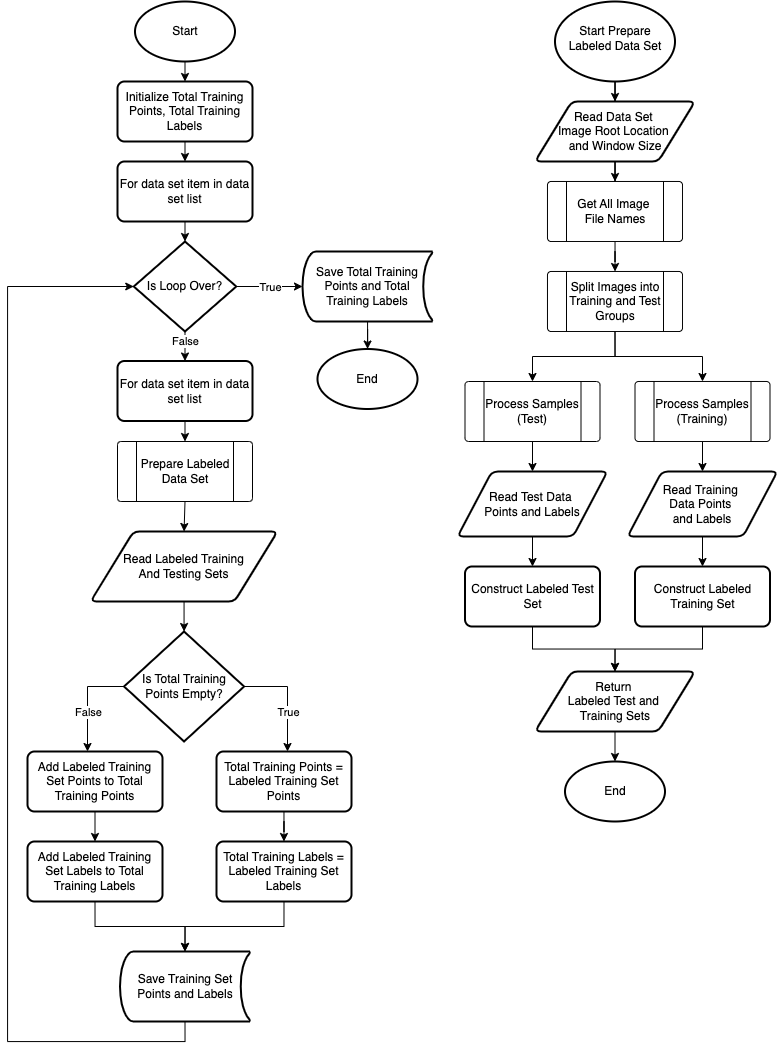
\includegraphics[width=0.75\linewidth]{images/ee_dataset_high.drawio.png}
    \caption{A high level overview flowchart of the process of initializing and saving the total training points and labels alongside each data set's testing points and labels}
    \label{fig:dataset_high}
\end{figure}

A major concern, however, has been raised with per-window evaluation: the scheme often relies on the use of cropped positives (windows where a pedestrian is neatly bounded) and uncropped negatives (windows that are not specifically cropped to contain random objects or background scenery). Classifiers may exploit this window boundary effect as discriminative features leading to poor real-world generalization \cite{dollar_2009_pedestrian}.

This concern is addressed to some degree in appendix \ref{appendix:dataset} by applying random value paddings to the bounding boxes that comprise positive samples. This process is further explained in figure \ref{fig:dataset_low}.

\begin{figure}
    \centering
    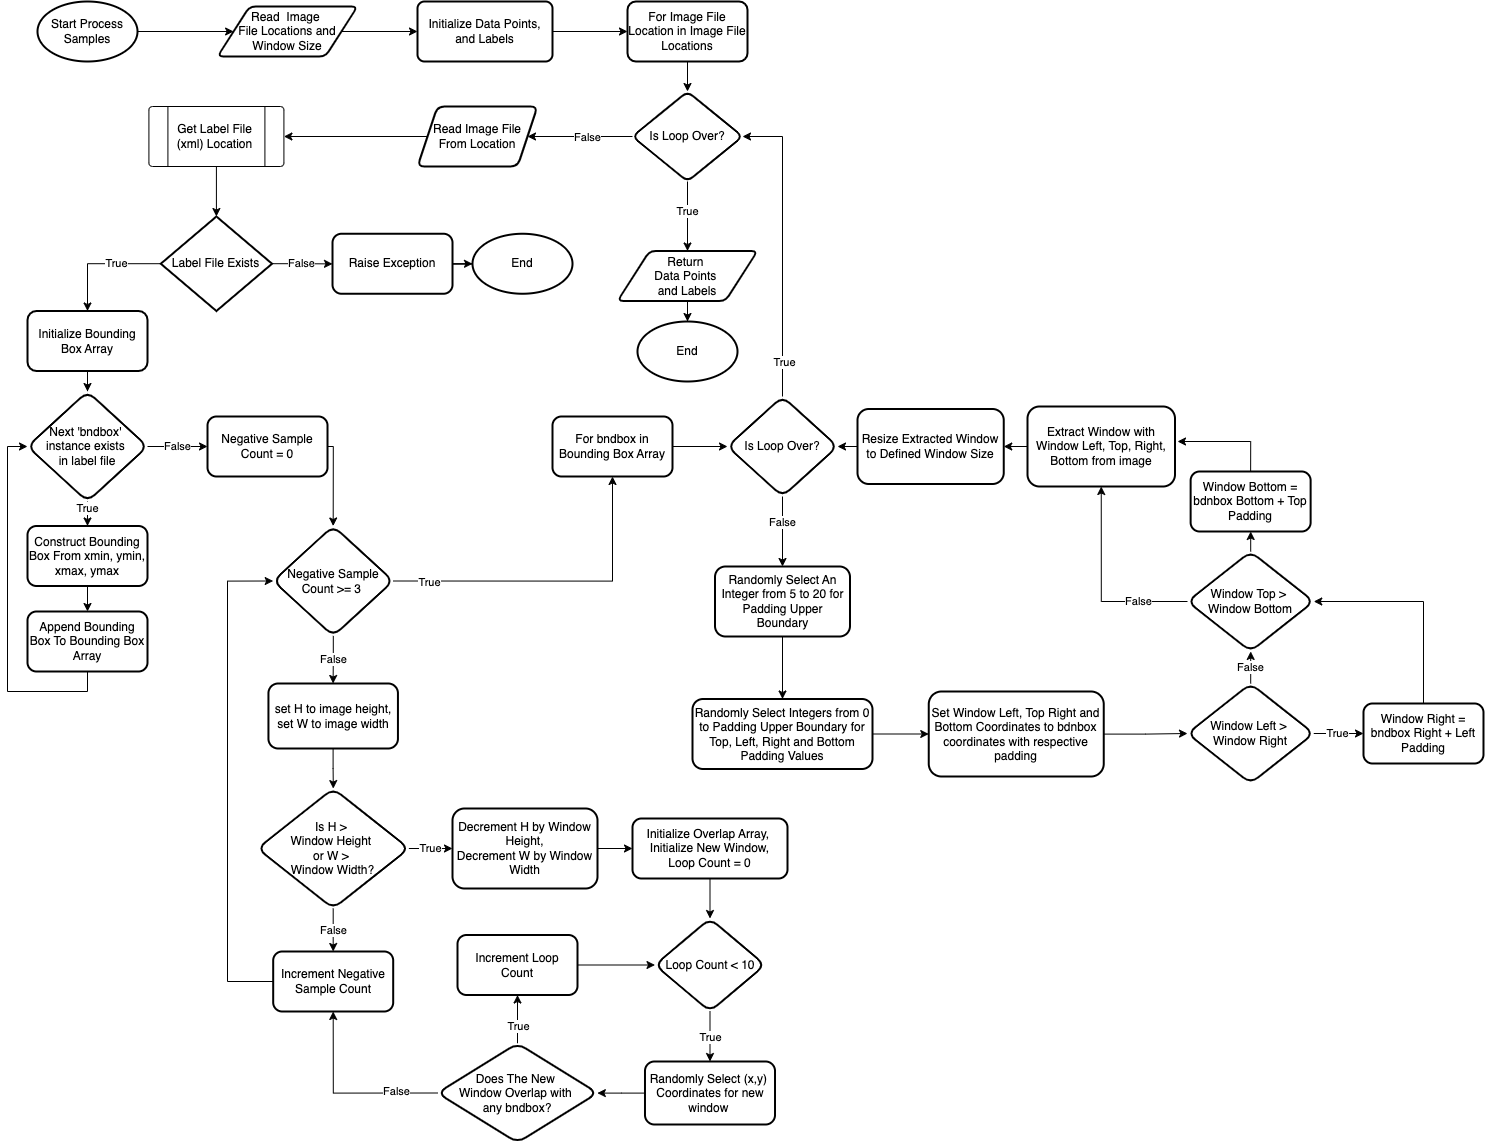
\includegraphics[width=\linewidth]{images/ee_dataset_low.drawio (1).png}
    \caption{A flowchart of the process of extracting the positive data samples (with some degree of random padding to avoid cropped positive bias) and the process of constructing negative samples }
    \label{fig:dataset_low}
\end{figure}

By using an 80/20\% training-testing data split, the number of images from section \ref{sec:caltech_trasnform} yields the numbers of different window size samples in table \ref{table:window_size_samples}

\begin{table}[H]    
    \begin{minipage}{.5\linewidth}
    \renewcommand{\arraystretch}{1.0}
    \centering
        \begin{tabular}{@{} l @{\hspace{0.5cm}} l @{\hspace{0.5cm}} l @{}}    
            \toprule
            \emph{Window Set} & \emph{Positive} & \emph{Negative}  \\\midrule
            INRIA Testing & 361 & 543  \\ 
            Caltech Testing & 2195 & 2558  \\ 
            PnPLO Testing & 596 & 578  \\
            Total Training & 12794 & 14760 \\\bottomrule
        \end{tabular}
        \subcaption{Window Size (100, 50)}
    \end{minipage}%
    \begin{minipage}{.5\linewidth}
    \renewcommand{\arraystretch}{1.0}
    \centering
        \begin{tabular}{@{} l @{\hspace{0.5cm}} l @{\hspace{0.5cm}} l @{}}    
            \toprule
            \emph{Window Set} & \emph{Positive} & \emph{Negative}  \\\midrule
            INRIA Testing & 361 & 533  \\ 
            Caltech Testing & 2195 & 2548  \\ 
            PnPLO Testing & 596 & 475  \\
            Total Training & 12794 & 14185 \\\bottomrule
        \end{tabular}
        \subcaption{Window Size (128, 96)}
    \end{minipage}%

    \vspace{1cm} % Space between rows of mini pages

    \begin{minipage}{.5\linewidth}
    \renewcommand{\arraystretch}{1.0}
    \centering
        \begin{tabular}{@{} l @{\hspace{0.5cm}} l @{\hspace{0.5cm}} l @{}}    
            \toprule
            \emph{Window Set} & \emph{Positive} & \emph{Negative}  \\\midrule
            INRIA Testing & 361 & 540  \\ 
            Caltech Testing & 2195 & 2554  \\ 
            PnPLO Testing & 596 & 535  \\
            Total Training & 12794 & 14511 \\\bottomrule
        \end{tabular}
        \subcaption{Window Size (128, 64)}
    \end{minipage}%
    \begin{minipage}{.5\linewidth}
    \renewcommand{\arraystretch}{1.0}
    \centering
        \begin{tabular}{@{} l @{\hspace{0.5cm}} l @{\hspace{0.5cm}} l @{}}    
            \toprule
            \emph{Window Set} & \emph{Positive} & \emph{Negative}  \\\midrule
            INRIA Testing & 361 & 543  \\ 
            Caltech Testing & 2195 & 2558  \\ 
            PnPLO Testing & 596 & 574  \\
            Total Training & 12794 & 14731 \\\bottomrule
        \end{tabular}
        \subcaption{Window Size (112, 48)}
    \end{minipage}%
\caption{Positive And Negative Window Samples For Each Data Set at Each Window Size.}
\label{table:window_size_samples}
\end{table}
\subsection{Model Preparation}

A dataset is prepared for each set of dependent variables in two steps: 
\begin{enumerate}
    \item Preprocessing each window sample
    \item Computing the HOG features
\end{enumerate}
\subsubsection{Preprocessing: Grayscale Image Transformation}

The already modest impact of color space in HOG has been shown to be further reduced by the use of block normalization \cite{dalal_2005_histograms}. Thus, for the sake computational simplicity, images are converted to grayscale \cite{madk_2008_perceptual} using the color mapping in equation \ref{eq:colour_map}, which is discussed in appendix \ref{appendix:grayscale_discuss} and implemented in appendix \ref{appendix:grayscale}.

\begin{equation}\label{eq:colour_map}
    Y \leftarrow 0.2125 \cdot R + 0.7154 \cdot G + 0.0721 \cdot B
\end{equation}

\subsubsection{Computing HOG Features}

Since neither the \href{https://scikit-image.org/}{scikit-image} nor \href{https://opencv.org/}{OpenCV} libraries provide an implementation of HOG which would allow changing block stride values, a custom implementation of the algorithm can be found in appendix \ref{appendix:hog}, with figure \ref{fig:hog_flowchart} providing a technical overview. The two parts of the hog pipeline (from figure \ref{fig:hog_pipeline}) that have been reused from \href{https://scikit-image.org/}{scikit-image} are orientation binning and block normalization. This is primarily because both parts are highly optimized using \href{https://cython.org/}{Cython}. Even while the gradients are not distributed using equation \ref{eq:bin}, giving a time complexity of $\mathcal{O}(\omega \cdot c_h \cdot c_w)$ instead of $\mathcal{O}(c_h \cdot c_w)$, the speed of the library's Cython implementation outperforms anything that's possible using regular python.

\begin{figure}
    \centering
    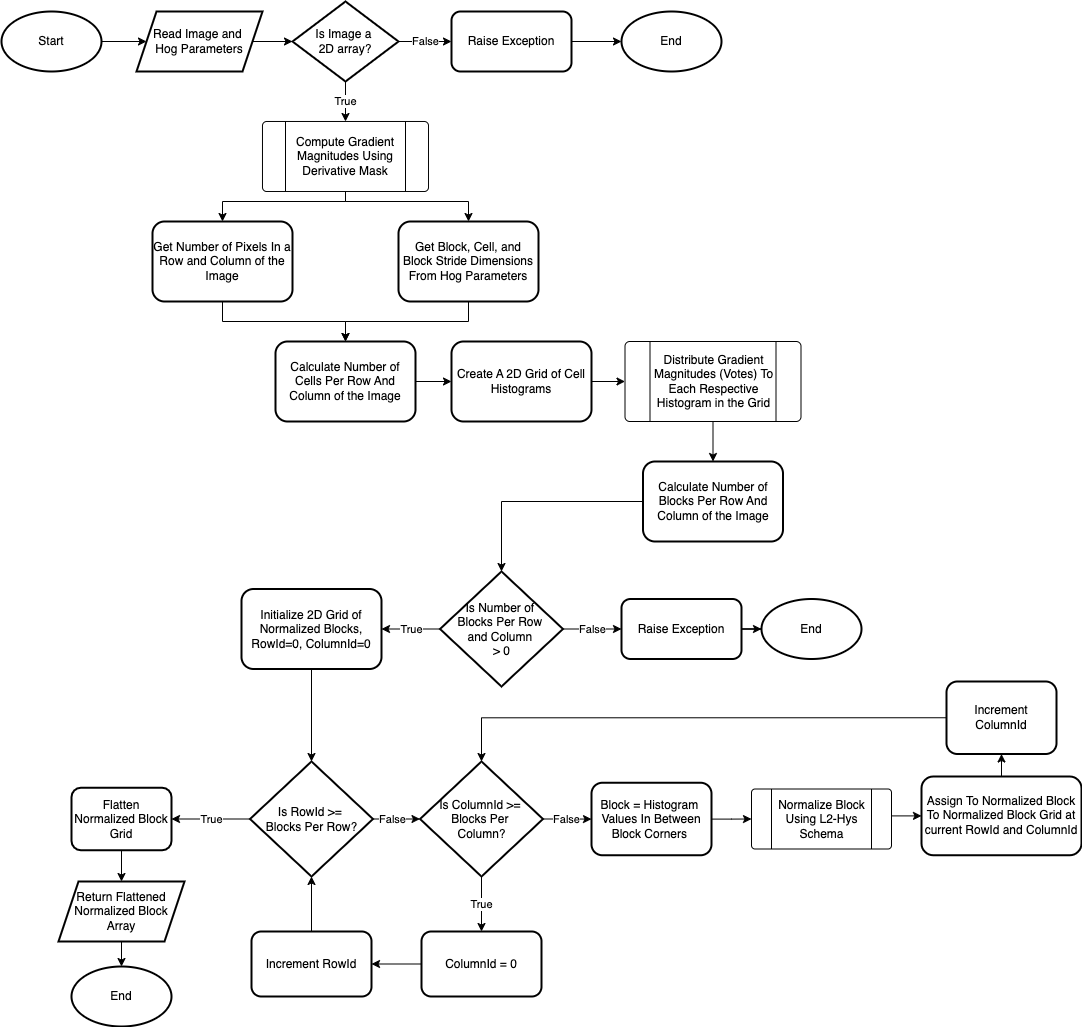
\includegraphics[width=0.85\linewidth]{images/ee_hog.drawio.png}
    \caption{A flowchart of the process of computing HOG features with custom block stride values}
    \label{fig:hog_flowchart}
\end{figure}

\subsubsection{Choosing an SVM}\label{sec:svm_choice}

Given the relatively large number of models that have to be trained on $\sim$ 27,000 samples, an implementation which reduces training time while maintaining decent performance is a necessity.

On larger datasets the maintainers of \href{https://scikit-learn.org/}{scikit-learn} recommend using either LibLinear \cite{linearsvc} or their implementation of a linear SVM with stochastic gradient descent (SGD) \cite{sgdclassifier} instead of the standard LibSVM \cite{chang_lin_2011_libsvm} (in practice it takes $\sim$ 1,600,000 \% more time to train an SVM with SMO as opposed to SGD \cite{sgd_leon})

SGD, in contrast to regular gradient descent (GD), only uses a subset of samples when determining the cost function's (with inputs of $||w||_{2}$ and $b$), gradient and the subsequent direction towards the global minima \cite{uc_berkeley_sgd}. As such, while having faster training times, SGD does not guarantee convergence to the global minima as well as GD does \cite{uc_berkeley_sgd}. In practice however, both LibLinear and an SVM with SGD exhibit essentially identical pedestrian classification performance, as evidenced by a McNemar's test p-value of $\sim$ 0.121, further comparisons are made in table \ref{tab:liblinear_vs_sgd_table} and figure \ref{fig:liblinear_vs_sgd_curve}.

\begin{table}
    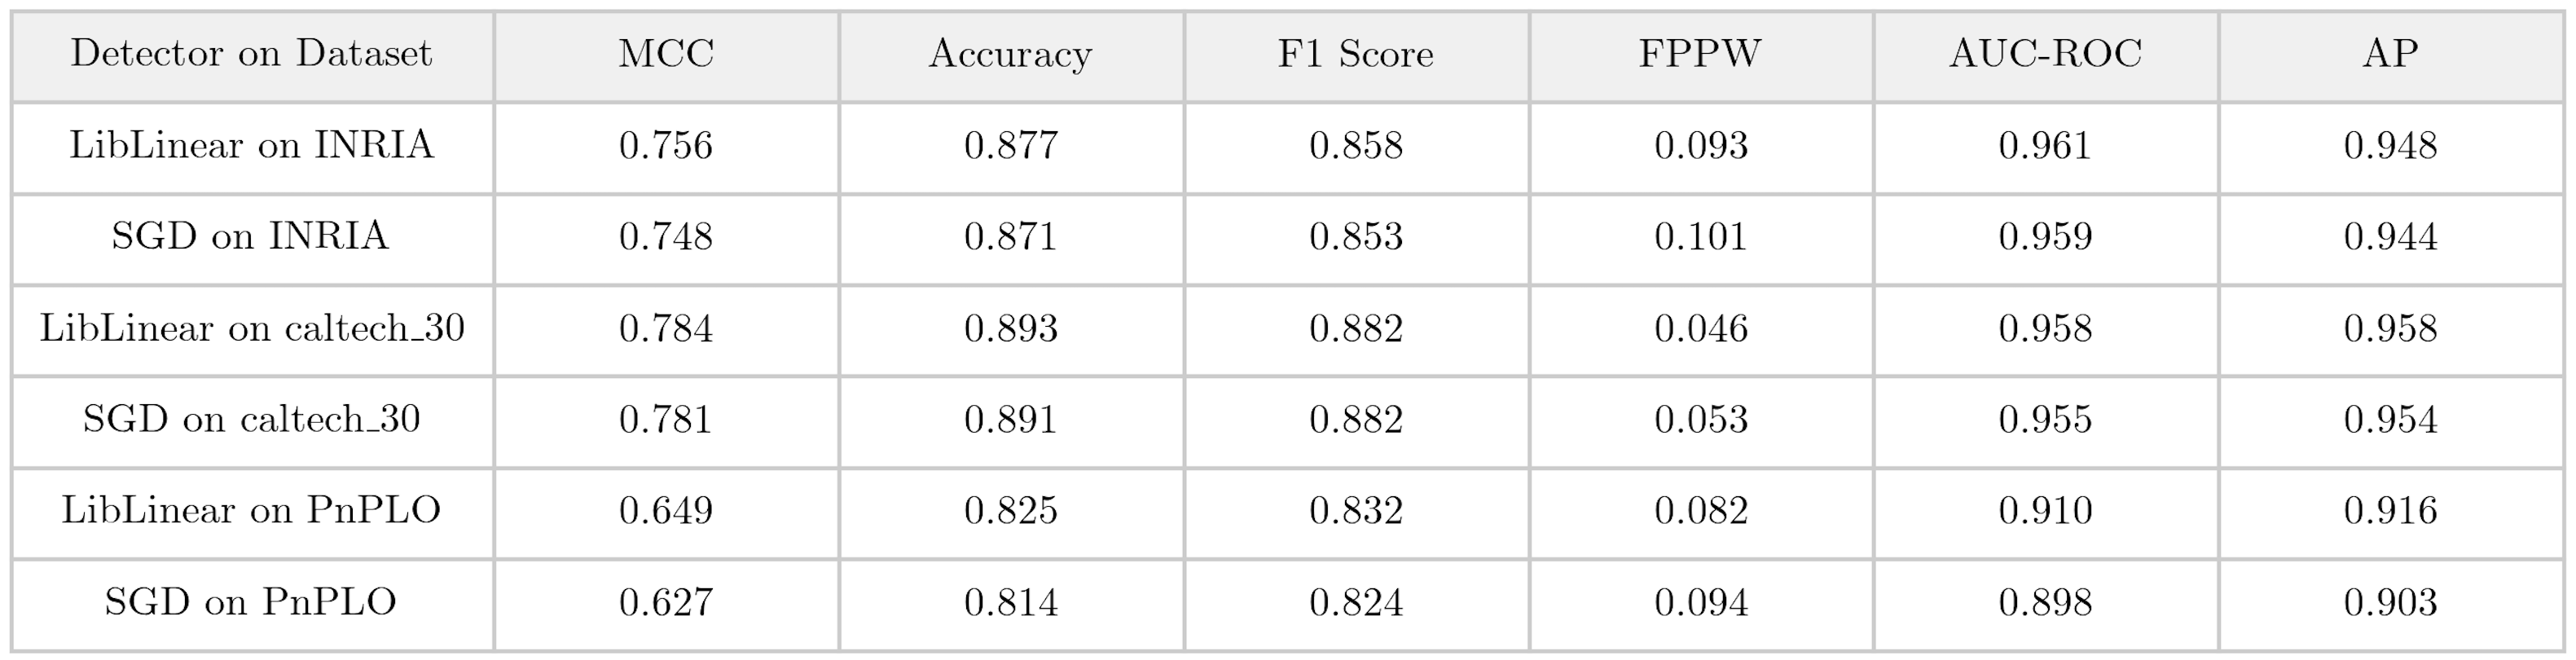
\includegraphics[width=\linewidth]{images/liblinear_vs_sgd_table.png}
    \caption{LinearSVC vs SGDClassifier evaluation scores on HOG features with standard parameters \cite{dalal_2005_histograms}: (128,64) window, (6,6) cell, (3,3) block sizes and (1,1) block strides. Code in appendix \ref{appendix:evaluate_metrics}}
    \label{tab:liblinear_vs_sgd_table}. 
\end{table}


\begin{figure}
    \centering
    \includesvg[width=0.75\linewidth]{images/liblinear_vs_sgd_curve.svg}
    \caption{An MCC-F1 curve of both LinearSVC and SGDClassifier trained on the standard HOG feature parameters \cite{dalal_2005_histograms}. \protect\footnotemark}
    \label{fig:liblinear_vs_sgd_curve}
\end{figure}

\footnotetext{Notice that the best performing $\tau$ value for SGDClassifier is negative, as $\tau$ identifies the distance which allows a point to be classified as a positive. This relates to Soft Constraint SVMs discussed in section \ref{sec:soft_constraint_svm}.}

\subsubsection{Training an SVM}

The code in appendix \ref{appendix:training_svm} implements SVM training using SGDClassifier optimized through cross 5-fold validation (with GridSearchCV) \cite{cornell_hyperoptimization}, which systematically explores four different soft regularization strength values (alpha). The grid search results in 20 fits from which the best performing model (in terms of MCC) is saved. While the initial learning rate (eta$\theta$) should also be optimized, this investigation avoids additional training overhead by using Leon Bottou's "optimal heuristic" for deriving the learning rate from alpha \cite{sgd_leon}.

The majority of the training was performed on a linux-based system with an Intel Xeon CPU @ 2.20GHz (2 cores), 12.7GB of RAM, as provided by \href{https://colab.research.google.com/}{Google Colab}. Since high dimensional HOG features (from figure \ref{fig:dimension_distribution}) tend to exceed the memory capacity of google colab's free tier, the training for higher dimensional models was done on a local machine with an Intel Core i7 @ 2.6GHz (6 cores) and 32GB of RAM.

\begin{figure}
    \includesvg[
        width=\linewidth,
    ]{dimension_distribution.svg}
    \caption{Kernel Density Estimation (KDE) of Dimension Values generated from various HOG parameters. The most frequent number of dimensions is 3780, which is the number of dimensions for the standard HOG parameters \cite{dalal_2005_histograms}.}
    \label{fig:dimension_distribution}
\end{figure}